% !TEX root = ../main.tex
% =====================================================================
% 3. PROPOSED METHODS
%
% Everything I designed: the SEA-Net encoder, its variants, the MIL
% pooling heads and the training objective. Notation is the one defined
% once in Table 1 and is not repeated here.
% =====================================================================

\section{Proposed Methods}
\label{sec:methods}

\begin{contribution}
The encoder family, the pooling heads and the training objective described in this section are my
own design and implementation. They keep the two-stage MIL template of \Cref{sec:bg:millet} --
encoder, then pooling head -- and the same tensor interface as \millet{}, so that every comparison
in \Cref{sec:results} isolates one component at a time.
\end{contribution}

I refer to the proposed architecture as \seanet{}, for \emph{Selective Evidence Aggregation
Network}, because it combines multi-scale temporal feature extraction with selective, class-specific
aggregation of the evidence found at each time step. A complete \seanet{} model is always the pair
\emph{encoder $+$ pooling head}. Five design goals, fixed before implementation, motivate the
choices that follow. \textbf{G1, small}: substantially fewer parameters than InceptionTime, at a
scale compatible with a microcontroller target. \textbf{G2, at least as accurate}, under an
identical training configuration. \textbf{G3, length-preserving}: one embedding per time step at
every stage, because the interpretation has one value per time step and AOPCR masks individual time
steps, so $\nsteps$ must never change inside the encoder. \textbf{G4, local}: each embedding must
depend on a bounded window of the input, otherwise the importance map becomes diffuse and
uninformative. \textbf{G5, modular}: encoder and pooling head selectable from a configuration file,
so any pair can be trained without modifying code.

% =====================================================================
\subsection{The \seanet{} encoder}
\label{sec:methods:encoder}

\Cref{fig:arch_overall} gives an overview of the encoder and of its interface with the pooling head;
only the design choices behind it are discussed here.

The encoder is a stem convolution, which lifts the single input channel to $\dmodel$ channels,
followed by a stack of \emph{multi-scale separable residual blocks} (\Cref{sec:arch:block}). Three
choices matter. Every convolution uses ``same'' zero padding with no stride and no pooling, so the
time axis is preserved end to end and the encoder returns exactly the per-time-step embeddings
$\emb_j$ that \Cref{eq:encoder_generic} requires (goal~G3). The dilation grows geometrically from
block to block, $\delta_i = \min(2^i, \delta_{\max})$, but is capped at $\delta_{\max} = 16$, so the
receptive field widens quickly in the early blocks and then stops, keeping each embedding tied to a
bounded window (goal~G4). Finally, encoder and head communicate through one fixed contract: the
encoder consumes $(B, 1, \nsteps)$ and returns $(B, \dmodel, \nsteps)$, and the head returns the
prediction $(B, \nclz)$ and the interpretation $(B, \nclz, \nsteps)$. Every variant and every head
below respects that contract, which is what makes the combinations of \Cref{sec:results} possible
from configuration alone (goal~G5).

% Source of truth for the figure: seanet/features.py (MSTCNSepEncoder, MultiScaleSepBlock),
% seanet/model.py (EncoderPoolNet), configs/models/sv2/seanet.yaml (d=128, n_blocks=6,
% kernels {5,11,23}, max_dilation=16, dropout=0.2). The small variants used in Section 5 are
% d=64, n_blocks=4.
\begin{figure}[t]
  \centering
  \makebox[\linewidth][c]{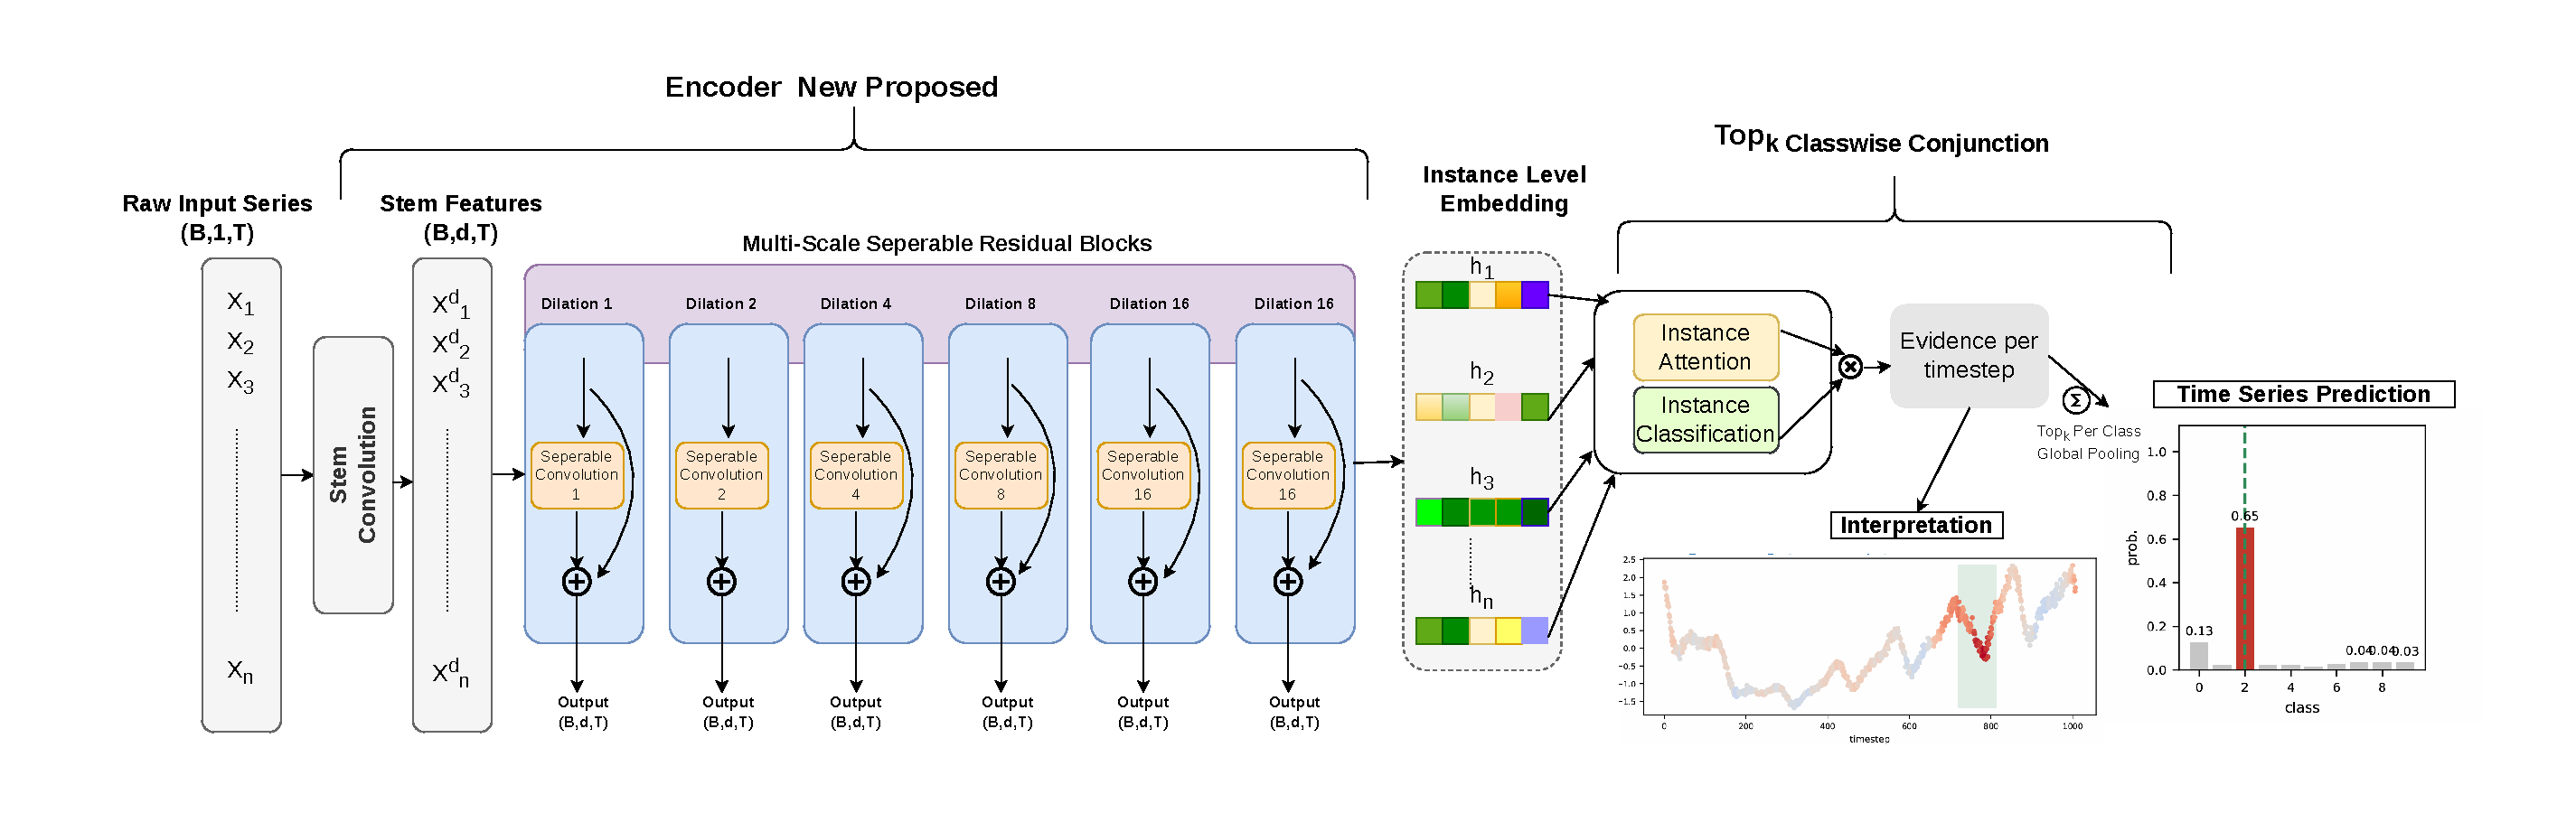
\includegraphics[width=1.0\linewidth]{figures/fig04_seanet_architecture.pdf}}
  \caption{Overview of a complete \seanet{} model, read left to right, with the tensor shape under
  each stage. \textbf{Left, the \seanet{} encoder:} the series $(B,1,\nsteps)$ passes through a stem
  convolution to $(B,\dmodel,\nsteps)$ and then through six multi-scale separable residual blocks,
  whose dilation grows $1,2,4,8$ and is then capped at $16$; the curved arrow inside each block is
  the residual connection, and $\nsteps$ is unchanged at every stage. \textbf{Middle:} one
  instance-level embedding $\emb_j$ per time step. \textbf{Right, the MIL pooling head
  (\Cref{sec:methods:pooling}):} an attention branch scores how much each time step counts, a
  classifier branch scores what it argues for, and their product is the evidence at that time step.
  Aggregating the evidence over time gives the prediction (bar chart); retaining the same
  per-time-step evidence gives the interpretation drawn on the series. The explanation and the
  prediction are the same quantities.}
  \label{fig:arch_overall}
\end{figure}

% =====================================================================
\subsection{The multi-scale separable block}
\label{sec:arch:block}

The block combines two established ideas with one addition. \emph{Dilated} convolutions
\citep{bai2018tcn} space the filter taps apart, so the window widens without extra weights.
\emph{Depthwise-separable} convolutions \citep{chollet2017xception, howard2017mobilenets} factorise
one convolution into a depthwise step $D_k^{(\delta)}$, which filters each channel independently
along time, and a pointwise $1\times1$ step $P$, which mixes channels at one time step. The addition
is that three kernel sizes run in parallel inside every block. One \emph{unit} chains the two steps
and one block runs two units and adds the input back:
\begin{equation}
  \mathcal{U}(\mathbf{h})
  = \operatorname{Drop}\Big(\operatorname{ReLU}\Big(\operatorname{BN}\Big(
      P\Big(\textstyle\sum_{k \in \mathcal{K}} D_k^{(\delta)}(\mathbf{h})\Big)\Big)\Big)\Big),
  \qquad \mathcal{K} = \{5, 11, 23\},
  \label{eq:unit}
\end{equation}
\begin{equation}
  \operatorname{Block}(\mathbf{h}) = \operatorname{ReLU}\big(\mathbf{h} +
  (\mathcal{U} \circ \mathcal{U})(\mathbf{h})\big).
  \label{eq:block}
\end{equation}

\Cref{eq:unit} examines the same signal at three time scales simultaneously: a kernel of size 5
covers a narrow local pattern, a kernel of size 23 reaches about four times further, and their
outputs are summed, so the block never has to commit to one scale in advance. The pointwise
convolution $P$ then combines what the three kernels found, BatchNorm \citep{ioffe2015batchnorm}
keeps activations on a stable scale, ReLU provides the non-linearity and dropout regularises. The
residual connection in \Cref{eq:block} makes the block an identity plus a correction, which keeps
deep stacks trainable.

\paragraph{Why the block is small.}
A standard convolution with $\dmodel$ input and output channels and kernel size $k$ costs
$\dmodel^2 k$ weights, whereas a depthwise-separable pair costs only
\begin{equation}
  \underbrace{\dmodel k}_{\text{depthwise}} \;+\; \underbrace{\dmodel^2}_{\text{pointwise}}
  \;\ll\; \dmodel^2 k .
  \label{eq:sep_cost}
\end{equation}
Counting the weights of \Cref{eq:unit} at the wide setting $\dmodel = 128$, the three depthwise
convolutions cost $\dmodel(6 + 12 + 24) = 5{,}376$ weights including one bias per channel, while the
single pointwise convolution costs $\dmodel^2 + \dmodel = 16{,}512$ -- three times more than all
three depthwise convolutions combined. With BatchNorm's $2\dmodel$, one unit costs $22{,}144$
parameters, one block $44{,}288$, and the six-block encoder with its stem about $266{,}752$,
consistent with the $269{,}083$ measured for the wide base model. A non-separable convolution
covering the same three kernel sizes would cost $\dmodel^2(5{+}11{+}23) = 638{,}976$ weights for the
same step, roughly $29\times$ more. Two consequences follow: goal~G1 becomes reachable at all, and
the pointwise convolution now dominates the parameter count, which is what \Cref{sec:var:bottleneck}
attacks.

% This figure is OPTIONAL. It is drawn in TikZ in figures/fig_block_tikz.tex and switched by
% \showblockfigtrue / \showblockfigfalse in preamble.tex. Nothing in the running text cites
% \Cref{fig:arch_block} on purpose, so hiding it cannot leave a dangling reference.
\ifshowblockfig
\begin{figure}[t]
  \centering
  % !TEX root = ../main.tex
% =====================================================================
% fig_block_tikz.tex -- the zoom-in on ONE multi-scale separable block.
%
% Drawn in TikZ instead of an image file, so it stays sharp and so the
% numbers on it can never drift away from the text.
% Source of truth: seanet/features.py, class MultiScaleSepBlock.forward()
%
% This file is pulled in by sections/05_architecture.tex with \input, and
% that \input sits inside \ifshowblockfig ... \fi. So it is OPTIONAL:
% set \showblockfigfalse in preamble.tex and the whole thing disappears
% without touching anything else.
%
% Two panels:
%   (a) the data path through one unit, the "x2", and the residual add
%   (b) the receptive field: same 5 taps, dilation 1 against dilation 16
% =====================================================================

% ---- panel (a): the data path ---------------------------------------
\resizebox{\linewidth}{!}{%
\begin{tikzpicture}[
  font=\small,
  >={Stealth[length=2mm]},
  % a convolution branch: the three of them differ only in kernel size
  conv/.style   = {draw=orange!65!black, fill=orange!18, rounded corners=2pt,
                   minimum height=8mm, inner xsep=4pt, align=center},
  % the cheap "mix and clean up" steps after the sum
  stage/.style   = {draw=black!55, fill=black!7, rounded corners=2pt,
                   minimum height=8mm, minimum width=11mm, align=center},
  % the tensors going in and out
  tensor/.style = {draw=black!45, fill=black!3, rounded corners=2pt,
                   minimum height=11mm, minimum width=13mm, align=center},
  op/.style     = {draw=black!65, circle, inner sep=1pt, minimum size=5.5mm},
]

% --- input ------------------------------------------------------------
\node[tensor] (h) at (0,0) {$\mathbf{h}$\\[1pt]\scriptsize$(B,d,T)$};

% --- the three depthwise convolutions, one per kernel size ------------
% drawn with increasing width, so "wider box = looks further in time"
\node[conv, minimum width=20mm] (k5)  at (3.7, 1.7) {depthwise $k{=}5$\\[-1pt]\scriptsize dilation $\delta$, groups $=d$};
\node[conv, minimum width=26mm] (k11) at (3.7, 0.0) {depthwise $k{=}11$\\[-1pt]\scriptsize dilation $\delta$, groups $=d$};
\node[conv, minimum width=32mm] (k23) at (3.7,-1.7) {depthwise $k{=}23$\\[-1pt]\scriptsize dilation $\delta$, groups $=d$};

\draw[->] (h.east) -- ++(0.4,0) |- (k5.west);
\draw[->] (h.east) -- ++(0.4,0) |- (k11.west);
\draw[->] (h.east) -- ++(0.4,0) |- (k23.west);

% --- they are simply added together -----------------------------------
\node[op] (sum) at (6.9,0) {$+$};
\draw[->] (k5.east)  -| (sum.north);
\draw[->] (k11.east) -- (sum.west);
\draw[->] (k23.east) -| (sum.south);

% --- mix the channels, normalise, activate, regularise ----------------
\node[stage] (pw)   at ( 8.9,0) {$1{\times}1$\\[-1pt]pointwise};
\node[stage] (bn)   at (10.7,0) {BatchNorm};
\node[stage] (relu) at (12.4,0) {ReLU};
\node[stage] (drop) at (14.0,0) {Dropout};

\draw[->] (sum.east)  -- (pw.west);
\draw[->] (pw.east)   -- (bn.west);
\draw[->] (bn.east)   -- (relu.west);
\draw[->] (relu.east) -- (drop.west);

% --- the residual add that closes the block ---------------------------
\node[op] (add) at (16.0,0) {$+$};
\node[stage, minimum width=9mm] (outrelu) at (17.6,0) {ReLU};
\node[tensor] (out) at (19.6,0) {output\\[1pt]\scriptsize$(B,d,T)$};

\draw[->] (drop.east)     -- (add.west);
\draw[->] (add.east)      -- (outrelu.west);
\draw[->] (outrelu.east) -- (out.west);

% the skip connection: the BLOCK's own input, carried over the top
\draw[->, thick, black!60] (h.north) |- (0,3.0) -| node[pos=0.25, above, black!60]
      {\small skip connection: the block's own input $\mathbf{h}$} (add.north);

% --- the dashed box marking what gets repeated twice ------------------
\begin{scope}[on background layer]
  \node[draw=black!55, dashed, rounded corners=3pt, inner sep=7pt,
        fit=(k5)(k23)(drop)] (unitbox) {};
\end{scope}
% the label sits UNDER the dashed box, where nothing else is drawn
\node[anchor=north west, black!70] at ($(unitbox.south west)+(2pt,-1pt)$)
      {\small \textbf{one unit} -- run twice, back to back ($\times 2$)};

\end{tikzpicture}}

\vspace{5pt}

% ---- panel (b): the receptive field ---------------------------------
\resizebox{0.92\linewidth}{!}{%
\begin{tikzpicture}[x=0.185cm, y=1cm, font=\small, >={Stealth[length=1.6mm]}]

% ---- top row: dilation 1 --------------------------------------------
% 65 input positions; the k=5 filter takes 5 neighbouring points
\foreach \i in {0,...,64} { \fill[black!22] (\i,0) circle (0.5mm); }
\foreach \i in {30,31,32,33,34} {
  \draw[orange!65!black, thin] (\i,0) -- (32,0.85);
  \fill[orange!75!black] (\i,0) circle (0.9mm);
}
\fill[black!80] (32,0.85) circle (1.1mm);
\node[anchor=west, black!80] at (34,0.85) {\ one output value};
\node[anchor=east] at (-1.5,0) {$\delta = 1$\ };
\node[anchor=north, black!60] at (32,-0.30) {\small sees 5 time steps in a row};

% ---- bottom row: dilation 16 ----------------------------------------
\begin{scope}[yshift=-2.1cm]
\foreach \i in {0,...,64} { \fill[black!22] (\i,0) circle (0.5mm); }
\foreach \i in {0,16,32,48,64} {
  \draw[orange!65!black, thin] (\i,0) -- (32,0.85);
  \fill[orange!75!black] (\i,0) circle (0.9mm);
}
\fill[black!80] (32,0.85) circle (1.1mm);
\node[anchor=west, black!80] at (34,0.85) {\ one output value};
\node[anchor=east] at (-1.5,0) {$\delta = 16$\ };
\node[anchor=north, black!60] at (32,-0.30)
     {\small the same 5 taps, now spread over 65 time steps};
% the reach, drawn as a measured bar
\draw[<->, black!55] (0,-0.95) -- node[below, black!55, font=\small] {receptive field} (64,-0.95);
\end{scope}

\end{tikzpicture}}

  \caption{One multi-scale separable block. \emph{Top:} the data path of one unit -- three depthwise
  convolutions read the same input at kernel sizes 5, 11 and 23 and their outputs are summed, then a
  pointwise $1\times1$ convolution mixes the channels, followed by BatchNorm, ReLU and dropout.
  \emph{Bottom:} the effect of dilation. Both rows use the same five taps of the $k=5$ filter; at
  $\delta=1$ they span five neighbouring time steps, at $\delta=16$ the same five taps span 65.}
  \label{fig:arch_block}
\end{figure}
\fi

% =====================================================================
\subsection{\seanet{} encoder variants}
\label{sec:arch:variants}

Seven variants are built on the same block, each presented with the problem it addresses, the
modification in one equation, and its effect. Five are encoders in the strict sense; two are
\emph{wrappers} that sit in front of, or around, one of the encoders rather than replacing it. Every
variant modifies the pipeline at one of the four points shown in \Cref{fig:attach_points}, and each
diagram below is labelled with the point it uses.

\begin{figure}[htbp]
  \centering
  % !TEX root = ../main.tex
% The reference pipeline with the four places an encoder variant can plug in.
% Drawn once; every variant panel carries the letter of the zone it uses.
\resizebox{\linewidth}{!}{%
\begin{tikzpicture}[seavar]
  \node[io]  (mx)    at ( 0.6,0) {$\bag$};
  \node[blk] (mstem) at ( 3.0,0) {stem};
  \node[blk] (mblk)  at ( 5.9,0) {blocks};
  \node[io]  (mh)    at ( 8.6,0) {$\mathbf{h}$};
  \node[blk, dashed] (mpool) at (11.6,0) {pooling head};

  \draw[->] (mx.east)    -- (mstem.west);
  \draw[->] (mstem.east) -- (mblk.west);
  \draw[->] (mblk.east)  -- (mh.west);
  \draw[->] (mh.east)    -- (mpool.west);

  \node[zone] at (1.85, 0) {A};
  \node[zone] at (7.35, 0) {B};
  \node[zone] at ($(mblk.north east)+(0.12,0.10)$) {D};

  \begin{scope}[on background layer]
    \node[draw=black!60, dashed, rounded corners=3pt, inner sep=5pt,
          fit=(mstem)(mblk)(mh)] (cbox) {};
  \end{scope}
  \node[zone] at (cbox.north west) {C};

  \node[anchor=west, black!70] at (-0.2,-1.35)
    {\textbf{A} = before the stem \quad\textbullet\quad
     \textbf{B} = after the blocks, acting on $\mathbf{h}$ \quad\textbullet\quad
     \textbf{C} = wraps the whole encoder \quad\textbullet\quad
     \textbf{D} = inside every block};
\end{tikzpicture}}

  \caption{The reference \seanet{} pipeline and the four points at which an encoder variant can
  modify it. Every variant diagram below carries the letter of the point it uses.}
  \label{fig:attach_points}
\end{figure}

% ---------------------------------------------------------------------
\subsubsection{\seanet{} bottleneck encoder}
\label{sec:var:bottleneck}

\textbf{Problem.} The pointwise step dominates the parameter count, costing $\dmodel^2$ weights per
unit (\Cref{sec:arch:block}).

\textbf{Modification.} Factorise that $1\times1$ convolution into two cheaper ones through a narrow
middle layer of width $r = \dmodel/4$ -- squeeze $\dmodel \to r$, then expand $r \to \dmodel$:
\begin{equation}
  P = P_{\text{expand}} P_{\text{squeeze}}, \qquad
  P_{\text{squeeze}} \in \R^{r \times \dmodel}, \quad
  P_{\text{expand}} \in \R^{\dmodel \times r},
  \qquad \text{cost } \dmodel^2 \rightarrow 2\dmodel r .
  \label{eq:bottleneck}
\end{equation}

\textbf{Effect.} With $r = \dmodel/4$ the pointwise cost becomes $\dmodel^2/2$, exactly half,
independently of $\dmodel$. At the setting used in the experiments ($\dmodel = 64$, 4 blocks) this
reduces the complete model from 57{,}580 to 41{,}324 parameters -- a 28\,\% saving on the whole
encoder, not only on the pointwise step. The block still consumes and returns
$(B, \dmodel, \nsteps)$, so goals~G3 and~G5 are unaffected. This is the smallest encoder built here
and the one used in the headline result.

\begin{figure}[htbp]
  \centering
  % !TEX root = ../main.tex
% SEA-Net bottleneck encoder (zone D). Box heights are drawn to scale, so the
% narrow middle is visible rather than only stated.
\resizebox{\linewidth}{!}{%
\begin{tikzpicture}[seavar]
  \node[zone] at (12.6,0.9) {D};

  % --- the standard pointwise convolution, for comparison ---
  \node[side] (aL1) at (1.5, 0) {standard:\ };
  \node[chan, minimum height=12mm] (ac1) at (2.1, 0) {};
  \node[blk]                       (ap)  at (5.8, 0) {$1{\times}1$ pointwise, $\dmodel \to \dmodel$};
  \node[chan, minimum height=12mm] (ac2) at (9.5, 0) {};
  \node[anchor=west, black!75] at (10.2, 0) {cost $=\dmodel^2 = 4096$ weights};

  \draw[->] (ac1.east) -- (ap.west);
  \draw[->] (ap.east)  -- (ac2.west);
  \node[anchor=south, black!70, font=\scriptsize] at (ac1.north) {$\dmodel = 64$};
  \node[anchor=south, black!70, font=\scriptsize] at (ac2.north) {$\dmodel = 64$};

  % --- the bottleneck: same in, same out, narrow middle ---
  \node[side] (aL2) at (1.5,-2.0) {bottleneck:\ };
  \node[chan, minimum height=12mm] (ac3) at (2.1,-2.0) {};
  \node[new]                       (asq) at (4.0,-2.0) {squeeze\\[-1pt]$\dmodel \to r$};
  \node[chan, minimum height=3mm]  (ann) at (5.8,-2.0) {};   % 3mm = 12mm / 4, to scale
  \node[new]                       (aex) at (7.6,-2.0) {expand\\[-1pt]$r \to \dmodel$};
  \node[chan, minimum height=12mm] (ac4) at (9.5,-2.0) {};
  \node[anchor=west, black!75] at (10.2,-2.0) {cost $=2\dmodel r = \dmodel^2/2 = 2048$ weights};

  \draw[->] (ac3.east) -- (asq.west);
  \draw[->] (asq.east) -- (ann.west);
  \draw[->] (ann.east) -- (aex.west);
  \draw[->] (aex.east) -- (ac4.west);

  \node[anchor=south, black!70, font=\scriptsize] at (ac3.north) {$\dmodel = 64$};
  \node[anchor=south, black!70, font=\scriptsize] at (ac4.north) {$\dmodel = 64$};
  \node[anchor=south, black!70] at (5.8,-1.72) {$r = \dmodel/4 = 16$};
  \node[anchor=north, black!70, align=center] at (5.8,-2.75)
        {same input, same output -- only the middle is narrow (heights drawn to scale)};
\end{tikzpicture}}

  \caption{\seanet{} bottleneck encoder (point \textbf{D}). Top: the standard pointwise convolution.
  Bottom: the same input and output with a narrow middle layer. Heights are drawn to scale.}
  \label{fig:var_bottleneck}
\end{figure}

% ---------------------------------------------------------------------
\subsubsection{\seanet{} gated encoder}
\label{sec:var:gated}

\textbf{Problem.} Not every feature channel is informative for every series, but the base encoder
weights all channels equally.

\textbf{Modification.} After the blocks have produced $\mathbf{h}$, collapse the time axis into a
summary vector $\mathbf{s} \in \R^{\dmodel}$, convert it into a per-channel gate, and re-weight
every time step with it:
\begin{equation}
  \mathbf{s} = \operatorname{summary}_j(\mathbf{h}) ,
  \qquad
  \mathbf{g} = \sig(W_g\,\mathbf{s}) \in [0,1]^{\dmodel} ,
  \qquad
  \mathbf{h}'_j = \mathbf{h}_j \odot (1 + \mathbf{g}) .
  \label{eq:gate}
\end{equation}

\textbf{Effect.} Two details are deliberate. $\operatorname{summary}_j$ is one of three ways of
collapsing time -- maximum, mean or last time step -- and all three were trained under the same
configuration so they could be compared. The multiplier is $(1 + \mathbf{g}) \in [1,2]$ rather than
$\mathbf{g}$: a plain multiplication would let the gate drive features towards zero, whereas
amplifying on top of the original $\mathbf{h}$ preserves the differences between time steps, which
are exactly what AOPCR and NDCG@$n$ measure. The gate carries no time index, so it re-weights
channels and never affects the time axis.

% ---------------------------------------------------------------------
\subsubsection{\seanet{} input-gated encoder}
\label{sec:var:inputgate}

\textbf{Problem.} The gate of \Cref{eq:gate} is one vector for the entire series, so it cannot
express that a channel is informative in one part of the series and not in another.

\textbf{Modification.} Compute the gate directly from the raw input, so it varies with time:
\begin{equation}
  \mathbf{g}_j = \sig\!\big(W_g \ast \bag\big)_j \in [0,1]^{\dmodel},
  \qquad
  \mathbf{h}'_j = \mathbf{h}_j \odot (1 + \mathbf{g}_j) ,
  \label{eq:input_gate}
\end{equation}
where $W_g \ast \bag$ is a small convolution (kernel size 7) over the raw series.

\textbf{Effect.} The two variants differ only in the subscript: one gate for the whole series
computed from deep features, against one gate per time step computed from the raw signal. Training
both isolates the granularity of the gating mechanism, coarse against fine.

\begin{figure}[htbp]
  \centering
  \begin{subfigure}[t]{0.49\linewidth}
    \centering
    % !TEX root = ../main.tex
% SEA-Net gated encoder (zone B): one gate for the whole series, built from h.
\resizebox{\linewidth}{!}{%
\begin{tikzpicture}[seavar]
  \node[zone] at (8.2,0.75) {B};

  \node[io]  (bh)  at (0.3,0) {$\mathbf{h}$};
  \node[new] (bsm) at (2.7,-1.15) {summary over time\\[-1pt](max / mean / last)};
  \node[new] (bsg) at (5.2,-1.15) {$\sig(W_g\,\mathbf{s})$};
  \node[op]  (bmu) at (6.6,0) {$\odot$};
  \node[io]  (bho) at (7.7,0) {$\mathbf{h}'$};

  \draw[->] (bh.east)  -- (bmu.west);            % the main path stays straight
  \draw[->] (bh.south) |- (bsm.west);
  \draw[->] (bsm.east) -- (bsg.west);
  \draw[->] (bsg.east) -| (bmu.south);
  \draw[->] (bmu.east) -- (bho.west);
  \node[anchor=south, black!60] at (6.6,0.30) {$(1{+}\mathbf{g})$};
\end{tikzpicture}}

    \caption{\seanet{} gated encoder: one gate for the whole series, read from $\mathbf{h}$
    (\Cref{eq:gate}).}
    \label{fig:var_gated}
  \end{subfigure}\hfill
  \begin{subfigure}[t]{0.49\linewidth}
    \centering
    % !TEX root = ../main.tex
% SEA-Net input-gated encoder (zone B): one gate per time step, built from the
% raw input instead of from the deep features.
\resizebox{\linewidth}{!}{%
\begin{tikzpicture}[seavar]
  \node[zone] at (7.9,0.75) {B};

  \node[io]  (ch)  at (0.3, 0)    {$\mathbf{h}$};
  \node[io]  (cx)  at (0.3,-1.15) {$\bag$};
  \node[new] (ccv) at (3.3,-1.15) {conv $k{=}7$, then $\sig$\\[-1pt]one gate \emph{per time step}};
  \node[op]  (cmu) at (6.3, 0)    {$\odot$};
  \node[io]  (cho) at (7.4, 0)    {$\mathbf{h}'$};

  \draw[->] (ch.east)  -- (cmu.west);
  \draw[->] (cx.east)  -- (ccv.west);
  \draw[->] (ccv.east) -| (cmu.south);
  \draw[->] (cmu.east) -- (cho.west);
  \node[anchor=south, black!60] at (6.3,0.30) {$(1{+}\mathbf{g}_j)$};
\end{tikzpicture}}

    \caption{\seanet{} input-gated encoder: one gate per time step, read from the raw input
    (\Cref{eq:input_gate}).}
    \label{fig:var_inputgate}
  \end{subfigure}
  \caption{The two gated \seanet{} encoders (point \textbf{B}). In both, the straight line through
  $\odot$ is the main path and the gate is a side branch, so neither can collapse the time axis.
  Orange marks what the variant adds, grey the unchanged encoder.}
  \label{fig:var_gates}
\end{figure}

% ---------------------------------------------------------------------
\subsubsection{\seanet{} spike/trend encoder}
\label{sec:var:spiketrend}

\textbf{Problem.} A stack of convolutions followed by normalisation is biased towards smooth,
sustained patterns, whereas some class evidence is a single sharp discontinuity.

\textbf{Modification.} Run an explicitly high-pass branch alongside the encoder and merge the two:
\begin{align}
  \text{spike}_j &= \operatorname{ReLU}\!\big(\operatorname{BN}(\operatorname{Conv}_3(
  \bag - \operatorname{avg}_w(\bag)))\big)_j \in \R^{d_{\text{spike}}} ,
  \label{eq:spike_branch}\\
  \mathbf{h}_j &= P\big([\text{Encoder}(\bag)_j \,;\, \text{spike}_j]\big),
  \qquad
  \mathbf{h}'_j = \mathbf{h}_j \odot (1 + \mathbf{g}) \ \text{ as in \Cref{eq:gate}} .
  \label{eq:spike_mix}
\end{align}

\textbf{Effect.} Subtracting a local moving average $\operatorname{avg}_w$ (window $w = 5$) leaves a
signal that is near zero on smooth stretches and large only at discontinuities; a kernel-3
convolution turns it into $d_{\text{spike}} = 16$ channels, concatenated with the trend features and
mixed back to width $\dmodel$. The expectation was an advantage on datasets with impulsive evidence.
\Cref{tab:ablation_encoder} shows this was the weakest of the five true encoders, so it was not met.

% ---------------------------------------------------------------------
\subsubsection{\seanet{} reconstruction-residual encoder}
\label{sec:var:recon}

\textbf{Problem.} The previous variant assumes in advance what the encoder misses. This one measures
it: which part of the input can the learned features \emph{not} account for?

\textbf{Modification.} A $1\times1$ convolution reconstructs the raw input from the trend features;
the reconstruction is subtracted from the real input and what remains becomes
$d_{\text{res}} = 16$ additional channels:
\begin{equation}
  \widehat{\bag} = P_{\text{rec}}(\text{trend}), \qquad
  \mathbf{h}_j = P\big([\,\text{trend}_j \,;\, \phi(\bag - \widehat{\bag})_j\,]\big),
  \label{eq:recon}
\end{equation}
with $\phi$ the same small convolution, BatchNorm and ReLU used for the spike branch.

\textbf{Effect.} The residual $\bag - \widehat{\bag}$ marks the parts of the signal the smooth
features cannot explain, a principled place to look for an unusual event. There is no separate
reconstruction loss: the branch is trained end to end, so it is a learned residual feature rather
than an auto-encoder. It was the second strongest encoder in \Cref{tab:ablation_encoder}.

\begin{figure}[htbp]
  \centering
  \begin{subfigure}[t]{0.49\linewidth}
    \centering
    % !TEX root = ../main.tex
% SEA-Net spike/trend encoder: a second high-pass branch off the raw input,
% merged back at zone B.
\resizebox{\linewidth}{!}{%
\begin{tikzpicture}[seavar]
  \node[zone] at (8.9,0.75) {B};

  \node[io]  (dx)  at (0.3,-0.5)  {$\bag$};
  \node[blk] (dtr) at (2.5, 0.30) {blocks \emph{(trend)}};
  \node[new] (dsp) at (2.5,-1.35) {$\bag - \operatorname{avg}_5$, conv$_3$ \emph{(spike)}};
  \node[new] (dmx) at (5.4,-0.5)  {mix $1{\times}1$};
  \node[new] (dg)  at (7.2,-0.5)  {gate};
  \node[io]  (do)  at (8.5,-0.5)  {$\mathbf{h}'$};

  \draw[->] (dx.east)  |- (dtr.west);
  \draw[->] (dx.east)  |- (dsp.west);
  \draw[->] (dtr.east) -| (dmx.north);
  \draw[->] (dsp.east) -| (dmx.south);
  \draw[->] (dmx.east) -- (dg.west);
  \draw[->] (dg.east)  -- (do.west);
\end{tikzpicture}}

    \caption{\seanet{} spike/trend encoder: a high-pass branch off the raw input
    (\Cref{eq:spike_branch}).}
    \label{fig:var_spiketrend}
  \end{subfigure}\hfill
  \begin{subfigure}[t]{0.49\linewidth}
    \centering
    % !TEX root = ../main.tex
% SEA-Net reconstruction-residual encoder: rebuild the input from the features,
% subtract it, and feed what is left back in at zone B.
\resizebox{\linewidth}{!}{%
\begin{tikzpicture}[seavar]
  \node[zone] at (9.4,0.75) {B};

  \node[io]  (eh)  at (0.3, 0.30) {$\mathbf{h}$};
  \node[new] (erb) at (2.2,-1.15) {rebuild $\widehat{\bag}$};
  \node[op]  (emn) at (3.9,-1.15) {$-$};
  \node[io]  (ex)  at (3.9,-2.20) {$\bag$};
  \node[new] (eph) at (6.0,-1.15) {$\phi$};
  \node[new] (emx) at (7.6, 0.30) {mix $1{\times}1$};
  \node[io]  (eo)  at (8.9, 0.30) {$\mathbf{h}'$};

  \draw[->] (eh.east)  -- (emx.west);
  \draw[->] (eh.south) |- (erb.west);
  \draw[->] (erb.east) -- (emn.west);
  \draw[->] (ex.north) -- (emn.south);
  \draw[->] (emn.east) -- node[above, black!60, inner sep=1pt] {$\bag-\widehat{\bag}$} (eph.west);
  \draw[->] (eph.east) -| (emx.south);
  \draw[->] (emx.east) -- (eo.west);
\end{tikzpicture}}

    \caption{\seanet{} reconstruction-residual encoder: a branch off $\mathbf{h}$
    (\Cref{eq:recon}).}
    \label{fig:var_recon}
  \end{subfigure}
  \caption{The two two-branch \seanet{} encoders (point \textbf{B}): the spike/trend encoder
  branches off the raw input to capture discontinuities, the reconstruction-residual encoder
  branches off the features to capture what they failed to rebuild.}
  \label{fig:var_branches}
\end{figure}

% ---------------------------------------------------------------------
\subsubsection{\seanet{} multi-scale channels (wrapper)}
\label{sec:var:mschan}

\textbf{Problem.} The stem receives a single raw channel, so any local statistic it needs must be
learned from scratch.

\textbf{Modification.} Append rolling maximum, minimum and standard deviation over several windows,
plus the sign of the first difference, as extra input channels:
\begin{equation}
  \bag^{+} = \Big[\, \bag \,;\; \big(\text{roll\_max}_w(\bag)\big)_{w \in \mathcal{W}} \;;\;
  \big(\text{roll\_min}_w(\bag)\big)_{w \in \mathcal{W}} \;;\;
  \big(\text{roll\_std}_w(\bag)\big)_{w \in \mathcal{W}} \;;\; \operatorname{sign}(\Delta \bag) \,\Big] ,
  \label{eq:mschan}
\end{equation}
with $\mathcal{W} = \{3,7,15,31\}$ (all odd, so each window stays centred).

\textbf{Effect.} This is a wrapper, not an encoder: it widens the input from 1 to
$1 + 4 \cdot 3 + 1 = 14$ channels before any encoder above. Maximum, minimum and standard deviation
are used rather than a rolling mean deliberately -- a mean is linear, so the stem convolution could
learn it on its own, whereas the other three are non-linear and add information a convolution cannot
compute. A BatchNorm normalises the 14 channels first, because they do not share the scale of the
raw series; omitting it cost accuracy.

% ---------------------------------------------------------------------
\subsubsection{\seanet{} multi-scale pyramid (wrapper)}
\label{sec:var:pyramid}

\textbf{Problem.} The dilation cap bounds the receptive field, so evidence visible only over a long
span cannot be reached.

\textbf{Modification.} Run the same encoder on the series downsampled by 1, 2, 4 and 8, stretch the
outputs back to length $\nsteps$, and fuse them with attention over the scale axis:
\begin{equation}
  \mathbf{h}_j = \sum_{s \in \mathcal{S}} \alpha_j^{s} \, \mathbf{h}_j^{(s)} ,
  \qquad
  \alpha_j^{s} = \operatorname{softmax}_{s}\big(\text{score}(\mathbf{h}_j^{(s)})\big),
  \qquad \mathcal{S} = \{1,2,4,8\} .
  \label{eq:pyramid_fusion}
\end{equation}

\textbf{Effect.} The softmax normalises over \emph{scale} and never over time, so the per-time-step
signal AOPCR and NDCG@$n$ depend on is preserved, and one set of encoder weights is shared across
all scales, so the parameter count barely changes and the extra cost is compute (about $1.9\times$).
This is the one-dimensional analogue of multi-magnification whole-slide-image MIL
\citep{hashimoto2020msdamil}, and it was the weakest variant built (\Cref{tab:ablation_encoder}). It
also imposes a constraint: the wrapped encoder must be shallow enough that its receptive field does
not exceed $\nsteps / \max(\mathcal{S})$, or the coarsest scales collapse to a nearly constant
signal. The pyramid therefore uses a shallow two-block base, and the pipeline verifies this condition
automatically.

\begin{figure}[htbp]
  \centering
  \begin{subfigure}[t]{0.49\linewidth}
    \centering
    % !TEX root = ../main.tex
% SEA-Net multi-scale channels (zone A): a wrapper that widens the input with
% rolling statistics before the stem. It is not an encoder on its own.
\resizebox{\linewidth}{!}{%
\begin{tikzpicture}[seavar]
  \node[zone] at (9.3,1.0) {A};

  \node[io]  (fx)  at (0.3,0) {$\bag$};
  \node[new] (frl) at (2.9,0) {rolling max / min / std\\[-1pt]$w \in \{3,7,15,31\}$\\[-1pt]$+\ \operatorname{sign}(\Delta\bag)$};
  \node[new] (fbn) at (6.0,0) {14 channels\\[-1pt]+ BatchNorm};
  \node[blk] (fst) at (8.2,0) {stem \dots};

  \draw[->] (fx.east)  -- (frl.west);
  \draw[->] (frl.east) -- (fbn.west);
  \draw[->] (fbn.east) -- (fst.west);
\end{tikzpicture}}

    \caption{\seanet{} multi-scale channels: widens the input before the stem
    (\Cref{eq:mschan}).}
    \label{fig:var_mschan}
  \end{subfigure}\hfill
  \begin{subfigure}[t]{0.49\linewidth}
    \centering
    % !TEX root = ../main.tex
% SEA-Net multi-scale pyramid (zone C): a wrapper that runs the SAME encoder on
% four downsampled copies of the series and fuses the results over scale.
\resizebox{\linewidth}{!}{%
\begin{tikzpicture}[seavar]
  \node[zone] at (9.9,1.0) {C};

  \node[io]  (gx)  at (0.3,0) {$\bag$};
  \node[new] (gds) at (2.0,0) {downsample\\[-1pt]$1,2,4,8$};
  \node[blk] (gbe) at (4.7,0) {the \emph{same} encoder\\[-1pt](shared weights)};
  \node[new] (gfu) at (7.7,0) {stretch back to $\nsteps$,\\[-1pt]softmax over \emph{scale},\\[-1pt]then fuse};
  \node[io]  (go)  at (9.6,0) {$\mathbf{h}$};

  \draw[->] (gx.east)  -- (gds.west);
  \draw[->] (gds.east) -- (gbe.west);
  \draw[->] (gbe.east) -- (gfu.west);
  \draw[->] (gfu.east) -- (go.west);
\end{tikzpicture}}

    \caption{\seanet{} multi-scale pyramid: runs one shared encoder at four scales
    (\Cref{eq:pyramid_fusion}).}
    \label{fig:var_pyramid}
  \end{subfigure}
  \caption{The two \seanet{} wrappers. They are not encoders: the channel wrapper acts before the
  stem (point \textbf{A}) and the pyramid wrapper around the whole encoder (point \textbf{C}), and
  both delegate feature extraction to one of the encoders above.}
  \label{fig:var_wrappers}
\end{figure}

\paragraph{Alternatives considered and rejected.}
A \textbf{Transformer encoder} was rejected on two grounds: full self-attention costs
$\mathcal{O}(\nsteps^2)$ in time and memory, prohibitive for series of 1{,}000--1{,}500 points on
the target hardware, and unrestricted attention lets any output position draw on any input position,
contradicting goal~G4. \textbf{Pruning or quantising InceptionTime} would reduce size but not address
the structural problem of \Cref{sec:bg:tsc}: the model still ends in global average pooling, so it
would still require a post-hoc explainer -- which is also why \textbf{keeping a large backbone and
explaining it afterwards} was rejected (\Cref{sec:intro:sota}).

% =====================================================================
\subsection{MIL pooling heads}
\label{sec:methods:pooling}

\begin{contribution}
The seven pooling heads below were designed and implemented by me. Five
(\Cref{sec:pool:classwise}--\Cref{sec:pool:attnmax}) follow directly from limitations L1--L3 of
\Cref{sec:bg:millet}. The last two adapt mechanisms published for whole-slide image classification
\citep{ilse2018attention, li2021dsmil}; the transfer to time series, the per-class formulation and
the implementation are mine.
\end{contribution}

Every proposed head keeps the two-part template of conjunctive pooling: an attention branch that
decides \emph{where} to look, and a per-time-step classifier that decides \emph{what} each position
argues for,
\begin{equation}
  \instpred_j = W_c \emb_j + \mathbf{b}_c \in \R^{\nclz},
  \qquad
  \mathbf{a}_j = \mathcal{A}(\emb_j) ,
  \label{eq:common_template}
\end{equation}
so a head is fully specified by two choices: the shape of the attention branch $\mathcal{A}$
(slot~1) and the operator combining the $\nsteps$ evidence values $g_j^k$ into $\bagpred^{\,k}$
(slot~2). Only slot~2 distinguishes five of the seven heads: they keep the class-wise attention
branch and change how the $\nsteps$ evidence values are reduced to one number -- a plain mean, a
smooth weighting, a hard selection of the largest few, or a blend with the maximum. The two
diagrams that draw the shared template and compare the seven aggregators side by side on the same
evidence profile are in the repository documentation (\Cref{sec:setup:pipeline}).

For every head, $\interp$ is not produced by a separate branch: it is exactly the per-time-step,
per-class quantity that $\bagpred$ is built from -- \Cref{eq:cw_bag}, for instance, sets
$\interp_{k,j} = g_j^k$, the very term that is averaged to obtain $\bagpred^{\,k}$. The
implementation follows the same rule, deriving both outputs from one intermediate tensor. Computing
them independently would allow them to disagree, which is precisely the weakness of post-hoc
explainers (\Cref{sec:intro:sota}).

The heads are presented in the order of the limitations they address: \Cref{sec:pool:classwise}
addresses~L1, \Cref{sec:pool:softmax} addresses~L2, and
\Cref{sec:pool:adaptive}--\Cref{sec:pool:dsmil} address~L3 through five different aggregation
strategies.

% The two pooling diagrams (figures/fig_pool_template.tex and
% figures/fig_pool_aggregators.tex) were moved to the repository documentation: they cost most of
% a page each and the prose above already says what each head puts in the two slots. The files are
% kept, so putting either back is one \input away.

% ---------------------------------------------------------------------
\subsubsection{Class-wise conjunctive pooling}
\label{sec:pool:classwise}

\textbf{Limitation addressed: L1.} The single gate of \Cref{eq:conj_gate} must serve all classes.

\textbf{Change.} Produce one gate per class from the same attention network, giving it $\nclz$
outputs instead of one:
\begin{align}
  \mathbf{a}_j &= \sig\!\left(W_2 \tanh(W_1 \emb_j)\right) \in [0,1]^{\nclz},
  \qquad W_1 \in \R^{\dattn \times \dmodel},\; W_2 \in \R^{\nclz \times \dattn},
  \label{eq:cw_gate}\\
  g_j^k &= a_j^k \, \instpred_j^{\,k},
  \qquad
  \bagpred^{\,k} = \frac{1}{\nsteps}\sum_{j=1}^{\nsteps} g_j^k,
  \qquad
  \interp_{k,j} = g_j^k .
  \label{eq:cw_bag}
\end{align}
The cost is $(\nclz-1)(\dattn+1)$ extra weights, a widening of the last attention layer only.

\begin{property}[Strict generalisation]
\label{prop:cw}
If $a_j^k = a_j$ for every class $k$, \Cref{eq:cw_bag} reduces exactly to conjunctive pooling
\Cref{eq:conj_bag}; if $a_j^k \to 1$ it reduces to instance pooling.
\end{property}

\textbf{Expected benefit.} A time step can now support one class and simultaneously argue against
another, making the class-specific interpretation meaningful. By Property~\ref{prop:cw} the head can
only add capacity: in the worst case it reproduces the baseline exactly.

% ---------------------------------------------------------------------
\subsubsection{Softmax conjunctive pooling with a learnable sharpness}
\label{sec:pool:softmax}

\textbf{Limitation addressed: L2.} The unnormalised sigmoid gate makes the bag score depend on the
series length.

\textbf{Change.} Replace the sigmoid gate by a distribution over time, normalised by a softmax whose
sharpness is controlled by a learnable parameter $\tau > 0$:
\begin{align}
  \alpha_j^k &= \softmaxt\!\left(\frac{s_j^k}{\tau}\right)
              = \frac{\exp(s_j^k/\tau)}{\sum_{i=1}^{\nsteps}\exp(s_i^k/\tau)},
  \qquad s_j^k = \left(W_2 \tanh(W_1 \emb_j)\right)_k,
  \label{eq:sm_alpha}\\
  \bagpred^{\,k} &= \sum_{j=1}^{\nsteps} \alpha_j^k \, \instpred_j^{\,k},
  \qquad
  \interp_{k,j} = \alpha_j^k \, \instpred_j^{\,k}.
  \label{eq:sm_bag}
\end{align}
The parameter $\tau$ divides the scores before the softmax and so controls how concentrated the
resulting weights are: a large $\tau$ flattens them towards uniform, a small $\tau$ concentrates
them on the highest-scoring steps. It is stored as $\tau = \exp(\rho)$ with $\rho$ learnable, so it
stays strictly positive, and adds one weight.

\begin{property}[Interpolation between mean and max]
\label{prop:sm}
As $\tau \to \infty$, $\alpha_j^k \to 1/\nsteps$ and \Cref{eq:sm_bag} becomes a plain mean over
time; as $\tau \to 0$ it selects the single highest-scoring time step. Because the weights sum to
one, $\bagpred^{\,k}$ does not depend on $\nsteps$.
\end{property}

\textbf{Expected benefit.} Series of different lengths become comparable, which should matter most
on the \ucr{} archive, and the model learns how concentrated its attention should be.

% ---------------------------------------------------------------------
\subsubsection{Adaptive class-wise pooling}
\label{sec:pool:adaptive}

\textbf{Limitation addressed: L3.} The fixed mean is appropriate only when the evidence is spread
out; where it is a single short event a max-like aggregator is better, and no fixed operator can be
right for both.

\textbf{Change.} Keep the per-class gates of \Cref{eq:cw_gate} and aggregate with a learnable
sharpness $\beta_k \geq 0$ per class, as a numerically stable soft-argmax:
\begin{equation}
  \beta_k = \softplus(\theta_k), \quad
  w_j^k = \softmaxt\!\left(\beta_k \, g_j^k\right), \quad
  \bagpred^{\,k} = \sum_{j=1}^{\nsteps} w_j^k \, g_j^k,
  \quad
  \interp_{k,j} = g_j^k .
  \label{eq:ad_bag}
\end{equation}
It adds $\nclz$ weights over class-wise pooling.

\begin{property}[Learned mean--max aggregator]
\label{prop:ad}
$\beta_k \to 0$ gives $w_j^k \to 1/\nsteps$, that is, class-wise conjunctive pooling;
$\beta_k \to \infty$ gives $\bagpred^{\,k} \to \max_j g_j^k$. Since $\bagpred^{\,k}$ is always a
convex combination of the $g_j^k$, it stays within their range, which keeps training stable.
\end{property}

\textbf{Expected benefit.} The aggregation adapts per class and per dataset instead of being fixed.
$\beta_k$ is initialised small (0.3), so training starts close to the safe class-wise mean and the
optimiser sharpens it only where that reduces the loss.

% ---------------------------------------------------------------------
\subsubsection{Top-$k$ conjunctive pooling}
\label{sec:pool:topk}

\textbf{Limitation addressed: L3, directly.} On a series of hundreds of time steps most positions
are background, and averaging over all of them dilutes the few decisive ones.

\textbf{Change.} Average only the $k$ largest evidence values of each class, with $k$ a fixed
fraction $\kappa$ of the series length:
\begin{align}
  k &= \max\big(1, \lceil \kappa \nsteps \rceil\big),
  \qquad
  \mathcal{S}^k_{\text{top}} = \big\{\, j : g_j^k \text{ is among the } k
    \text{ largest of } (g_1^k,\dots,g_{\nsteps}^k) \,\big\},
  \label{eq:topk_set}\\
  \bagpred^{\,k} &= \frac{1}{k}\sum_{j \in \mathcal{S}^k_{\text{top}}} g_j^k,
  \qquad
  \interp_{k,j} = g_j^k .
  \label{eq:topk_bag}
\end{align}
$\kappa \in (0,1]$ is a hyperparameter rather than a weight, so this head adds no parameters over
class-wise pooling.

\begin{property}[Strict generalisation]
\label{prop:topk}
$\kappa = 1$ recovers class-wise conjunctive pooling exactly. For $\kappa < 1$ the gradient reaches
only the selected time steps, which concentrates the evidence.
\end{property}

\textbf{Expected benefit.} The prediction rests on a small, explicit set of time steps, so masking
exactly those steps should damage the model far more than masking the same number of random ones --
an improvement in explanation quality rather than in accuracy. \Cref{tab:ablation_topk} tests
Property~\ref{prop:topk} by varying $\kappa$, and this is the head used in the best models of
\Cref{sec:results}.

% ---------------------------------------------------------------------
\subsubsection{Attention-max pooling}
\label{sec:pool:attnmax}

\textbf{Limitation addressed: L3, as a control.} Adaptive class-wise pooling also removes the fixed
mean, but its soft-argmax still mixes in every time step to some degree. This head is the simplest
hard alternative, to test whether the smoother learned aggregator is justified.

\textbf{Change.} A learnable per-class blend of the mean and the maximum, adding $\nclz$ weights:
\begin{equation}
  \bagpred^{\,k} = (1-\lambda_k)\,\frac{1}{\nsteps}\sum_{j=1}^{\nsteps} g_j^k
                   \; + \; \lambda_k \max_{j} g_j^k ,
  \qquad \lambda_k = \sig(\theta_k) \in [0,1].
  \label{eq:attnmax}
\end{equation}

\begin{property}
\label{prop:attnmax}
$\lambda_k \to 0$ recovers class-wise conjunctive pooling; $\lambda_k \to 1$ gives max pooling. Each
class learns independently whether its evidence is sustained or impulsive.
\end{property}

\textbf{Expected benefit.} \Cref{eq:attnmax} and \Cref{eq:ad_bag} use the same per-class gate and
differ only in how they reduce it to one number, so comparing them isolates a single factor: soft
against hard selection.

% ---------------------------------------------------------------------
\subsubsection{Per-class gated attention}
\label{sec:pool:gated}

\begin{priorwork}
The gated attention mechanism is due to \citet{ilse2018attention} and is used in the multi-scale MIL
pipeline of \citet{hashimoto2020msdamil}, where a bag is a whole-slide image and an instance is an
image patch (\Cref{sec:bg:mil}).
\end{priorwork}

\textbf{Limitation addressed: L1 and L3, through a stronger attention branch.} The baseline gate is
a single $\tanh$ layer, which limits how selective it can be.

\textbf{Change.} Transfer gated attention to time series (bag = series, instance = time step) and
make it \emph{per class}, which the original formulation is not:
\begin{align}
  \mathbf{A}_j &= \tanh(V \emb_j) \odot \sig(U \emb_j) \in \R^{\dattn},
  \qquad V, U \in \R^{\dattn \times \dmodel},
  \label{eq:ga_features}\\
  \alpha_j^k &= \softmaxt\big((W \mathbf{A}_j)_k\big),
  \qquad
  \bagpred^{\,k} = \sum_{j=1}^{\nsteps} \alpha_j^k \, \instpred_j^{\,k},
  \qquad
  \interp_{k,j} = \alpha_j^k \, \instpred_j^{\,k}.
  \label{eq:ga_bag}
\end{align}
The $\tanh$ branch proposes candidate attention features and the $\sig$ branch decides which to
admit, so a feature is used only where the second branch judges it reliable. The cost is a second
$\dmodel \to \dattn$ layer, making this the most expensive proposed head.

\textbf{Expected benefit and a structural caveat.} A more selective gate should sharpen the
interpretation. However, unlike every other head here, this one has no blend parameter that recovers
conjunctive pooling, so no setting of its weights returns the baseline. \Cref{sec:disc:negative}
shows that this matters in practice.

% ---------------------------------------------------------------------
\subsubsection{Dual-stream conjunctive pooling}
\label{sec:pool:dsmil}

\begin{priorwork}
The two-stream mechanism is due to \citet{li2021dsmil} (DSMIL), again for whole-slide images: one
stream aggregates all instances, a second focuses on the most critical instance and on the instances
resembling it (\Cref{sec:bg:mil}).
\end{priorwork}

\textbf{Limitation addressed: L3, when the evidence is scattered.} A single decisive time step
should be able to dominate without the surrounding evidence being discarded.

\textbf{Change.} I removed the contrastive pre-training of \citet{li2021dsmil}, made the critical
instance and the query per class, and combined the two streams with a learnable blend starting at
the conjunctive baseline. Stream~A is the class-wise conjunctive mean of \Cref{eq:cw_bag};
stream~B locates the most supporting time step for each class, embeds a query for every time step,
and re-weights by similarity to that critical query:
\begin{align}
  m_k &= \argmax_{j} \; g_j^k ,
  \qquad
  \mathbf{q}_j = W_q \emb_j \in \R^{\dattn},
  \qquad
  U_j^k = \softmaxt\!\left(\langle \mathbf{q}_j, \mathbf{q}_{m_k}\rangle\right),
  \label{eq:ds_query}\\
  \bagpred^{\,k} &= (1-\lambda)\,\frac{1}{\nsteps}\sum_{j=1}^{\nsteps} g_j^k
                 + \lambda\,\sum_{j=1}^{\nsteps} U_j^k \, \instpred_j^{\,k},
  \qquad
  \interp_{k,j} = (1-\lambda)\, g_j^k + \lambda\, U_j^k \instpred_j^{\,k},
  \label{eq:ds_blend}
\end{align}
with a single learnable scalar $\lambda = \sig(\theta)$, initialised at $0.05$.

\begin{property}[Safe by construction]
\label{prop:ds}
$\lambda \to 0$ recovers class-wise conjunctive pooling. The interpretation uses the same blend as
the logit, so the explanation always matches the decision. Attention is computed only against the
single critical time step, so the cost is $\mathcal{O}(\nsteps \dattn \nclz)$ rather than
$\mathcal{O}(\nsteps^2)$.
\end{property}

\textbf{Expected benefit.} Property~\ref{prop:ds} suggests this head should never be worse than the
baseline, and it was designed specifically to improve AOPCR. \Cref{sec:disc:negative} shows it is in
fact the weakest head tested, and explains why a safety property that nothing in the training
objective drives the model towards is ineffective in practice.

% =====================================================================
\subsection{Training objective}
\label{sec:methods:loss}

Every model in this report is trained with the same objective, which has two terms:
\begin{equation}
  \mathcal{L} = \underbrace{\mathrm{CE}(\bagpred, y)}_{\text{classification}}
              + \lambda_{\text{focus}} \cdot
                \underbrace{\Big({-}\sum_{j=1}^{\nsteps} \bar a_j \log(\bar a_j + \epsilon)\Big)}_{\text{attention entropy}} .
  \label{eq:loss}
\end{equation}

\paragraph{Classification term.}
Cross-entropy between the bag logits and the true label, with \emph{label smoothing} at 0.13, which
replaces the one-hot target by one that puts $1-\varepsilon$ on the correct class and spreads
$\varepsilon$ over the others. This prevents the model from driving its logits to arbitrarily large
values in order to reach a probability of exactly one. That matters more here than in an ordinary
classifier, because the interpretation is built from those same logits: over-confident logits produce
importance maps whose scale is dominated by a few saturated values.

\paragraph{Attention entropy term.}
The entropy of the attention distribution returned by the pooling head, where $\bar a_j$ is that
attention averaged over classes (so $\bar a_j = \frac{1}{\nclz}\sum_k a_j^k$ for the class-wise
family) and $\epsilon$ avoids $\log 0$. Entropy measures how spread out a distribution is: attention
concentrated on a few time steps has \emph{low} entropy, attention spread evenly over the series has
\emph{high} entropy. Adding entropy to a loss that is minimised therefore pushes the model towards
concentrated attention.

This term exists for the interpretation, not for the classification. Without it, nothing prevents
the model from reaching a correct prediction using a small amount of attention spread over hundreds
of time steps; the prediction is then correct but the importance map is flat, and a reader cannot
tell where the evidence stops. With the term, the model must reach the same prediction using fewer
time steps, which is what makes the resulting map readable and what both AOPCR and NDCG@$n$ reward.
The trade-off was measured directly: \Cref{tab:ablation_focus} shows that switching the term off
improves accuracy by about one point while reducing both explanation metrics. The weight is
$\lambda_{\text{focus}} = 0.01$ for every \seanet{} model and $0$ for the \millet{} baseline, since
the term is a \seanet{} addition.
